\chapter{Сравнение производительности алгоритмов}

В теории игр сравнивать разные алгоритмы достаточно просто - можно посмотреть на награды, полученные алгоритмами за эпизод.
Дополнительных метрик и критериев для сравнения не требуется.

Но, блядь, если мы говорим про среды с несколькими агентами, то тут уже надо выбирать специальные алгоритмы. Ну, допустим, в игре один агент говорит другому, куда бежать, и второй бежит туда (на время). На картинке \ref{aboba} \cite{https://doi.org/10.48550/arxiv.1509.02971} видно, что классические алгоритмы не понимают, что надо сотрудничать, чтобы выиграть.
Еще стоит учесть, блять, что не все алгоритмы обучения с подкреплением обеспечивают сходимость к оптимальной стратегии. Имей в виду, что некоторые алгоритмы могут не дать тебе настоящей гарантии, что ты выиграешь. А вот обратное обучение - это уже другая тема, блядь. Там агент не получает никаких наград, и мне кажется, что это тоже интересно. В дальнейшем мы могли бы посмотреть на алгоритмы обратного обучения.

\begin{figure}[H]
	\centering
	\begin{subfigure}[b]{0.45\textwidth}
		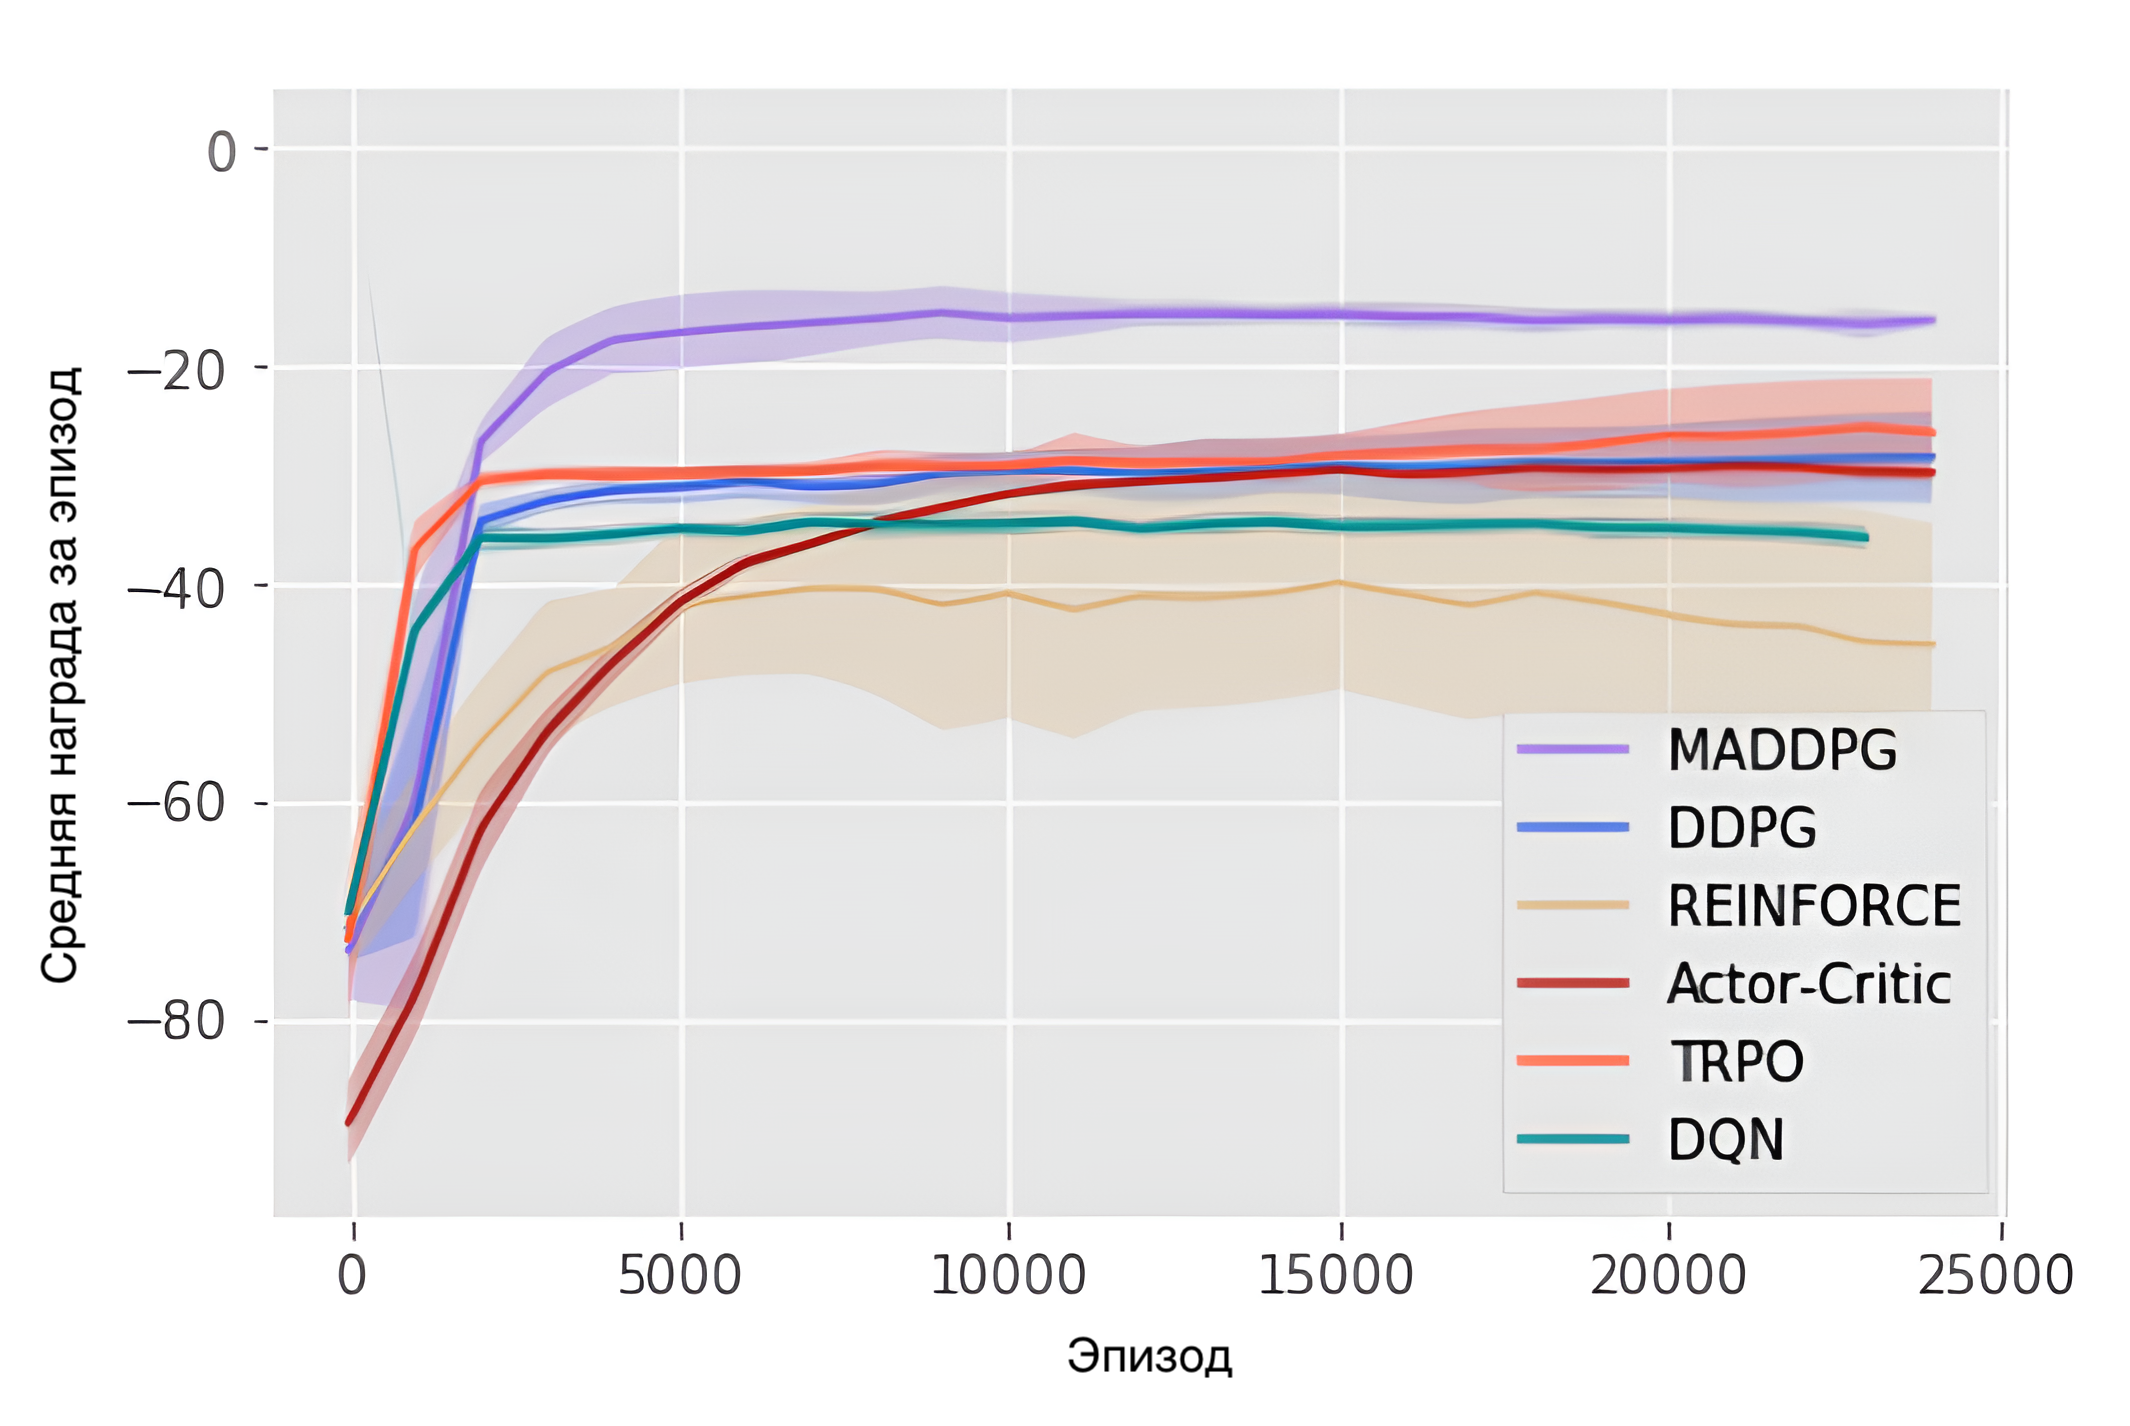
\includegraphics[width=\textwidth]{./inc/img/rl_vs_marl.png}
		\caption{Средняя награда за эпизод}
	\end{subfigure}
	\hfill
	\begin{subfigure}[b]{0.45\textwidth}
		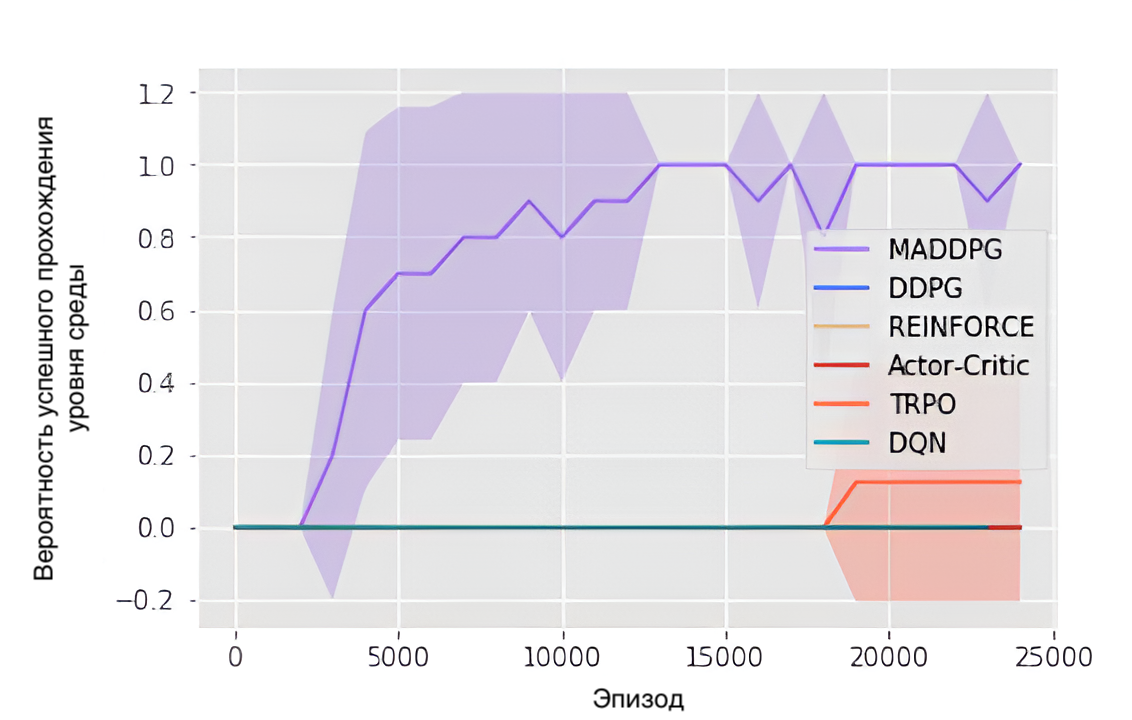
\includegraphics[width=\textwidth]{./inc/img/rl_vs_marl_2.png}
		\caption{Процент ситуаций, когда агент достигает цели}
	\end{subfigure}
	\caption{\centering Сравнение производительности MARL алгоритма MADDPG и классических RL алгоритмов}
	\label{aboba}
\end{figure}



\begin{figure}[H]
	\begin{center}
		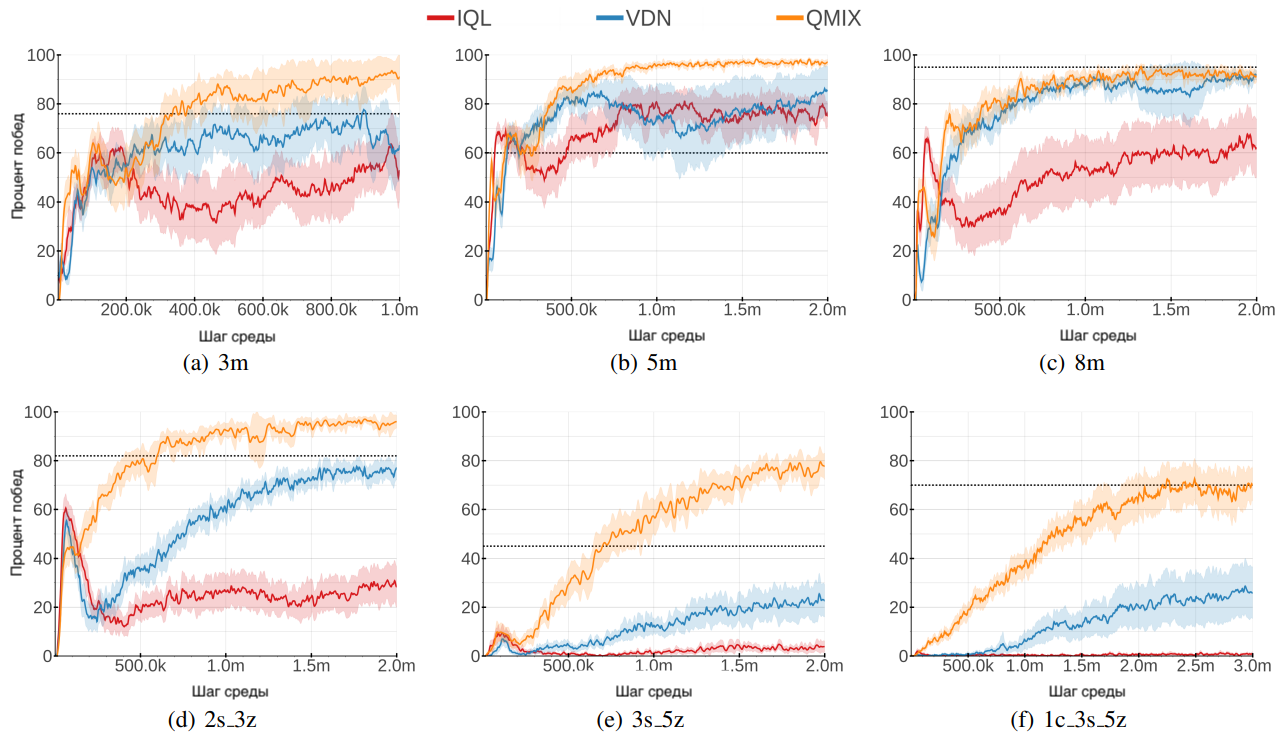
\includegraphics[pages=-, width=140mm]{./inc/img/qmix_winrate.png}
		\caption{Сравнение процента побед QMIX, VDN, IQL в среде StarCraft II в зависимости от кол--ва эпизодов для обучения}
		\label{fig:qmix_winrate}
	\end{center}
\end{figure}

Бля, смотри, ка, эти алгоритмы типа КОМА и КьюТран, они похожи на КьюМИКС, и поэтому их обсуждать - чистый шлак. Так что их показатели успеха практически нулевые, по сравнению с теми алгоритмами, что на \ref{fig:maven_winrate} показаны, ага. \cite{DBLP:journals/corr/abs-1910-07483}.

\begin{figure}[H]
	\begin{center}
		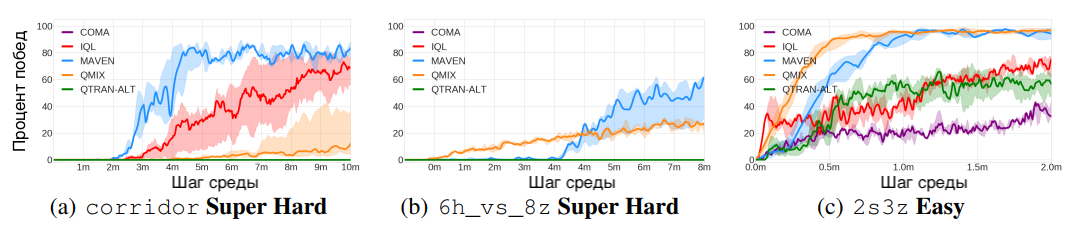
\includegraphics[pages=-, width=140mm]{./inc/img/maven_winrate.png}
		\caption{Сравнение процента побед MAVEN, QMIX, IQL, COMA, QTRAN, в среде StarCraft II в зависимости от кол--ва эпизодов для обучения}
		\label{fig:maven_winrate}
	\end{center}
\end{figure}

Похуй, но это говно-алгоритм MAVEN и QMIX крутят всех нахуй во всех категориях. Особенно кайфово использовать MAVEN в SMAC(StarCraft II), т. к. там пространство действий похуй какое огромное и надо его нормально исследовать \cite{DBLP:journals/corr/abs-1910-07483}.
%\begin{figure}[H]
%	\begin{center}
%	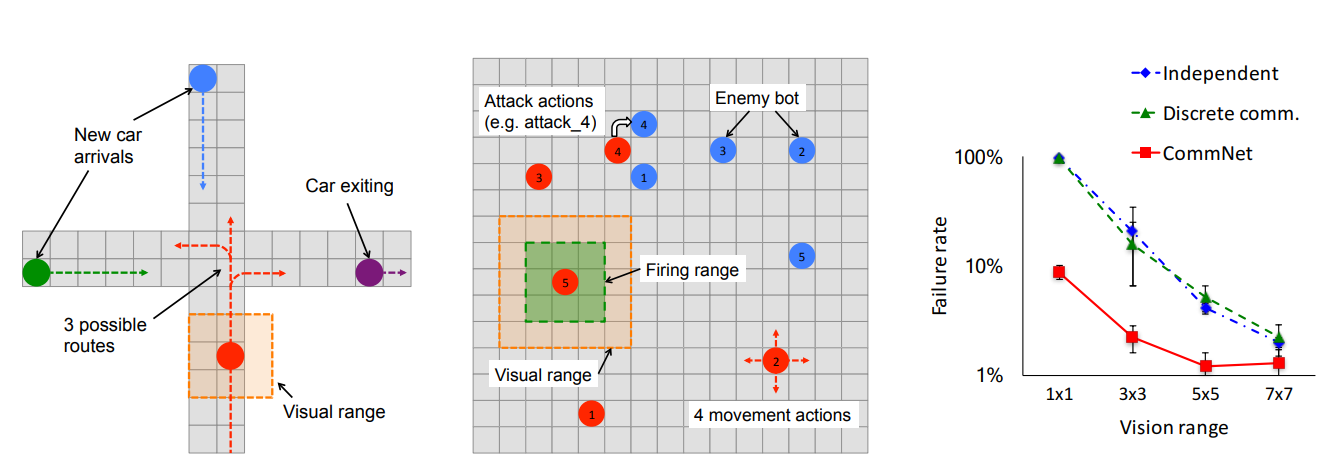
\includegraphics[pages=-, width=140mm]{./inc/img/commnet_perf.png}
%	\caption{Процент неудач в среде CrossRoad (слева) в зависимости от поля видимости для агентов управляемых независимыми сетями и алгоритмом CommNet}
%	\label{fig:commnet_perf}
%\end{center}
%\end{figure}

\begin{figure}[H]
	\begin{center}
		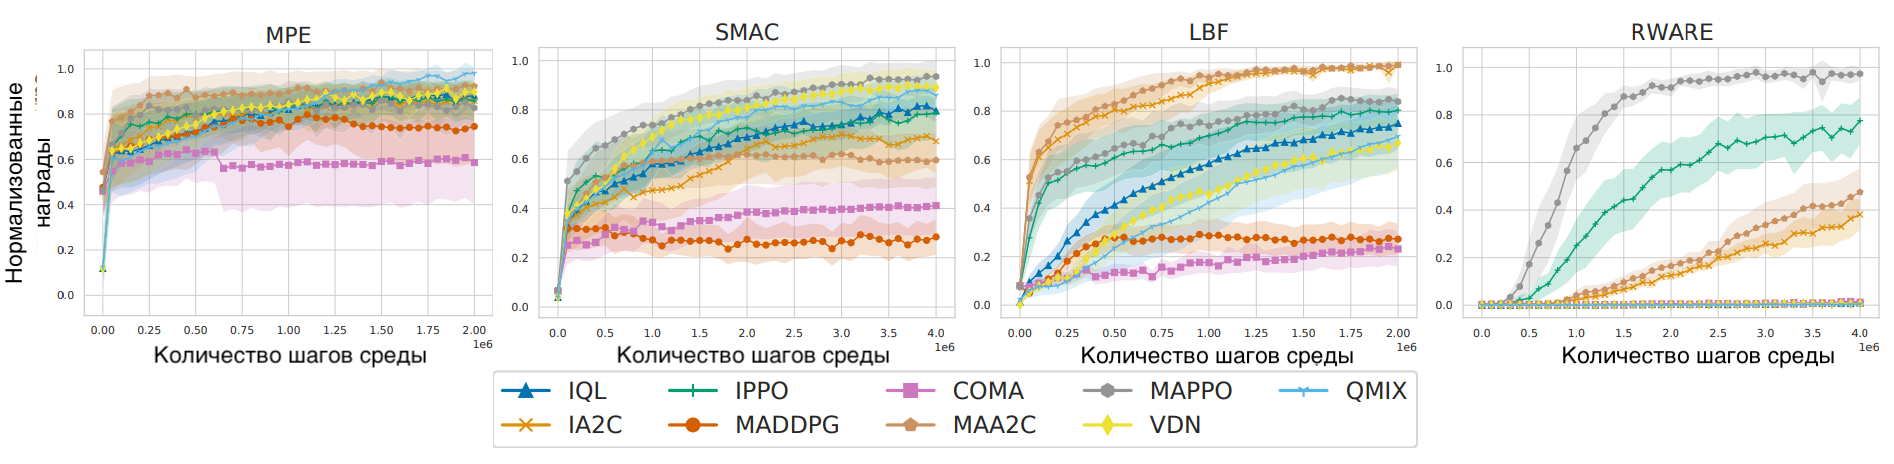
\includegraphics[pages=-, width=140mm]{./inc/img/comp_big.png}
		\caption{Нормализованное вознаграждение разных алгоритмов в на разных средах в зависимости от кол--ва эпизодов для обучения}
		\label{fig:mappo_perf}
	\end{center}
\end{figure}
Чекаем фотку \ref{fig:mappo_perf} \cite{DBLP:journals/corr/abs-2103-01955}, там все игры на борту. И как показывает наша бандитская наука, MAPPO - это топчик в большинстве игр. А IPPO, он ваще без методов обучения гопов-агентов дает хорошие результаты в большинстве игр, это все было описано в статье \cite{DBLP:journals/corr/abs-2103-01955}.

Если говорить о классических алгоритмах, то их модификации под многопользовательскую среду дают средние результаты. Только вот в среде IBF A2C (и обычный и с централизованным обучением Q) показался наилучшим гоп-выбором.
\subsection*{Вывод}
Ну вот, дрочили мы здесь эти алгоритмы, смотрели на графики и метрики, сравнивали их как сучки. Но теперь можно с уверенностью сказать, что всё четко и правильно, потому что использовали доступные инструменты для сравнения. Без тупых шуток, всё ок.
